\documentclass{article}

\usepackage{array}
\usepackage{graphicx}

\begin{document}

\title{Week 11, Session 2 Problems}
\author{GSI: Caleb Eades}
\date{11/1}
\maketitle

\section{Circuits}

\subsection{Equivalent Resistance}

Find the equivalent resistance of this circuit. Note that it cannot be decomposed into series and parallel.

\begin{figure}[h]
	\begin{center}
	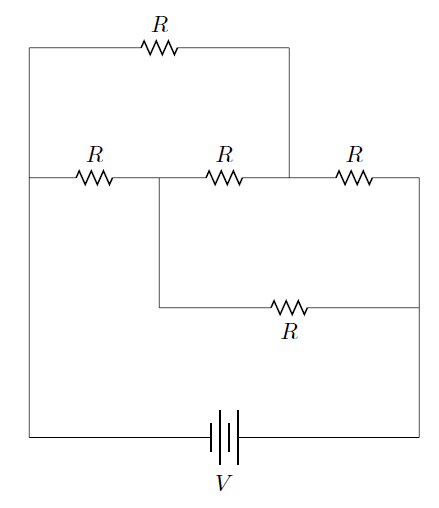
\includegraphics[width=0.5\textwidth]{Circuit.png}
	\end{center}
\end{figure}

(\textit{Source: Dan and Vetri})

\subsection{Kirchhoff Practice}

Consider the circuit shown. Suppose the current form A to B is 3 A.
\begin{itemize}
	\item[(a)] Find the current through each resistor.
	\item[(b)] Find the voltage V of the battery on the left.
	\item[(c)] Find the power generated by each battery.
\end{itemize}

\begin{figure}[h]
	\begin{center}
		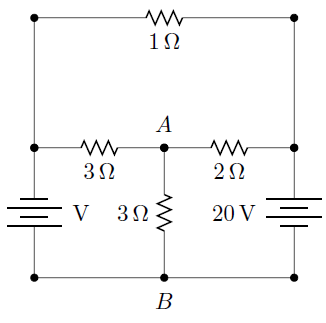
\includegraphics[width=0.5\textwidth]{PracticeCircuit.png}
	\end{center}
\end{figure}

(\textit{Source: http://physics.info/kirchhoff/practice.shtml})

\subsection{Capacitors in a Circuit}

Consider the circuit shown below that contains capacitors $C_1$ and $C_2$ and resistor $R$. Initially the switch is open and the capacitor $C_1$ has charge $Q_0$. The switch is closed at $t=0$.
\begin{itemize}
	\item[(a)] What is the initial current that flows through the resistor right after the switch is closed?
	\item[(b)] After a very long time, what are the charges $Q_1$ and $Q_2$ on $C_1$ and $C_2$ respectively?
	\item[(c)] What is the charge $Q_2(t)$ on $C_2$ as a function of time?
	\item[(d)] How will $Q_2(t)$ be modified if a dielectric of constant $\epsilon$ is inserted in between the plates of capacitor $C_2$?
\end{itemize}

\begin{figure}[h]
	\begin{center}
		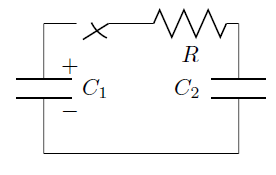
\includegraphics[width=0.5\textwidth]{CapacitorCircuit.png}
	\end{center}
\end{figure}

(\textit{Source: Lanzara Fall 2013 Midterm 2})

\subsection{}

Consider a circuit where a battery leads into a resistor $r$, which then splits into parallel resistors $r$ and $R$. If you wanted the power through the resistor $R$ to stay constant even if the resistance $R$ varies slightly, then what value of resistance $r$ should you use for the two other resistors in the circuit?

\end{document}
